\documentclass[a4paper]{article}
\usepackage[margin=0.8in]{geometry}
\usepackage{tikz}
\usepackage{xcolor}
\usetikzlibrary{arrows.meta, positioning, fit, backgrounds}

\definecolor{pri}{HTML}{0084FF}
\definecolor{red1}{HTML}{EF4444}
\definecolor{blue1}{HTML}{3B82F6}
\definecolor{green1}{HTML}{10B981}
\definecolor{amber1}{HTML}{E8920D}
\definecolor{dark}{HTML}{0F172A}
\definecolor{gray1}{HTML}{94A3B8}
\definecolor{mongo}{HTML}{00884A}
\definecolor{njs}{HTML}{4A8C3F}

\pagestyle{empty}

\begin{document}

\begin{center}
{\Large\bfseries\color{pri} ClinicQ Health Monitor --- System Block Diagram}\\[3pt]
{\small\color{gray1} Option 1: Dedicated ESP32 Per Patient ~|~ SEM6 Project}
\end{center}

\vspace{0.5cm}

\begin{center}
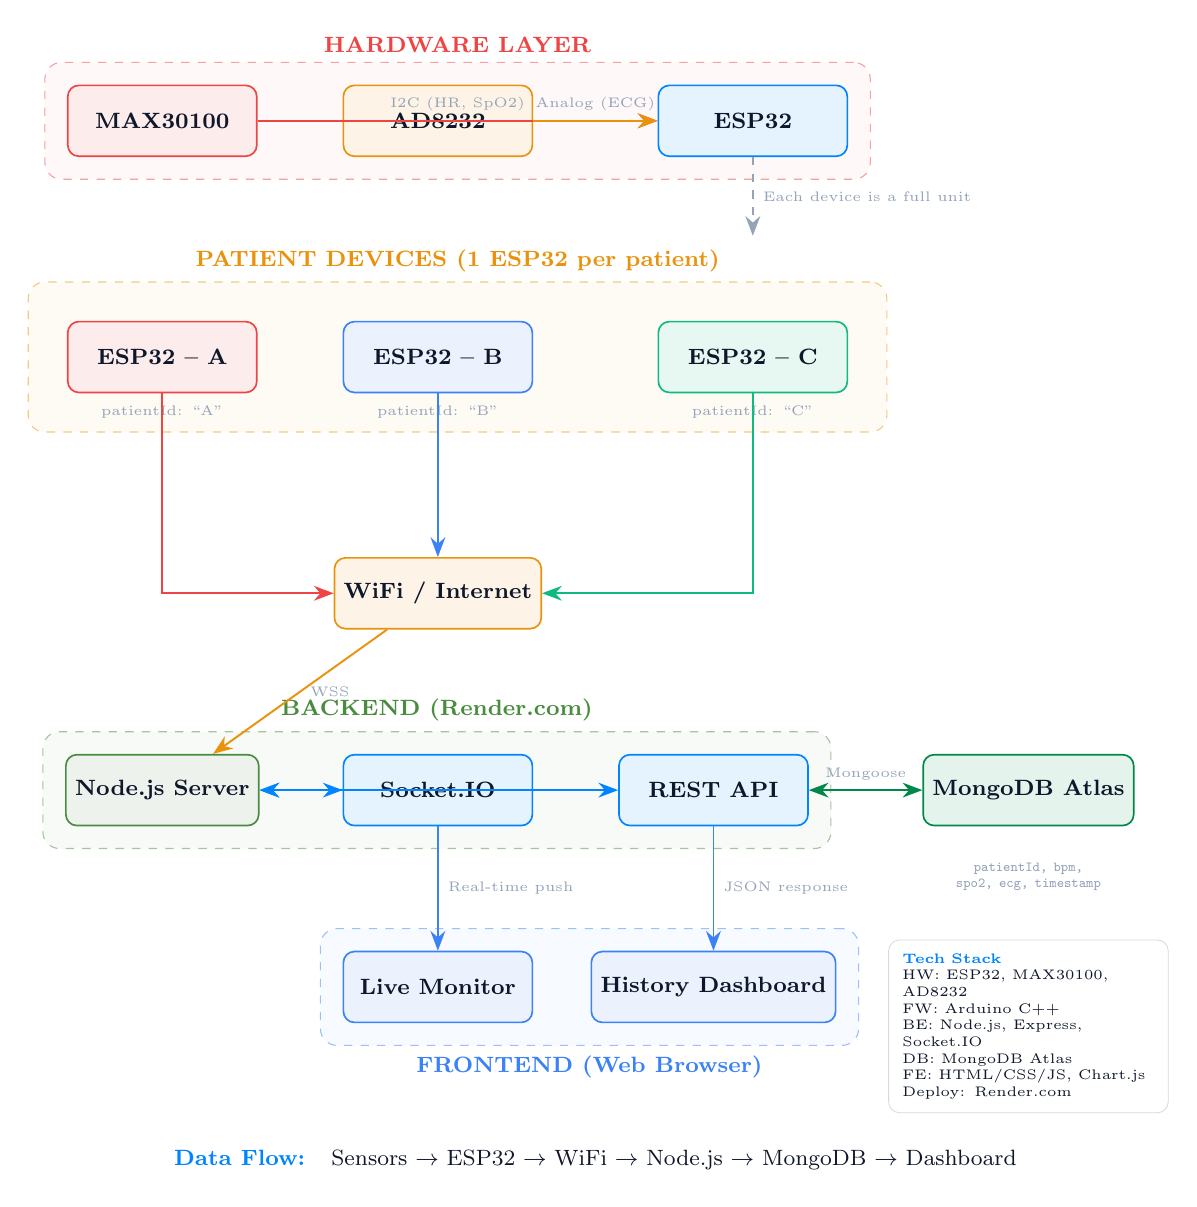
\begin{tikzpicture}[
    >={Stealth[length=2.5mm]},
    B/.style={rectangle, rounded corners=4pt, minimum width=2.4cm, minimum height=0.9cm,
              text centered, font=\footnotesize\bfseries, draw=#1, fill=#1!10, text=dark, line width=0.6pt},
    Z/.style={rectangle, rounded corners=6pt, draw=#1!50, fill=#1!4, line width=0.4pt, dashed, inner sep=8pt},
    A/.style={->, line width=0.7pt, color=#1},
    L/.style={font=\tiny, color=gray1, midway}
]

% === ROW 1: SENSORS ===
\node[B=red1] (s1) at (0,0) {MAX30100};
\node[B=amber1] (s2) at (3.5,0) {AD8232};
\node[B=pri] (esp) at (7.5,0) {ESP32};

\draw[A=red1] (s1) -- (esp) node[L,above] {I2C (HR, SpO2)};
\draw[A=amber1] (s2) -- (esp) node[L,above] {Analog (ECG)};

\begin{scope}[on background layer]
\node[Z=red1, fit=(s1)(s2)(esp), label={[font=\footnotesize\bfseries\color{red1}]above:HARDWARE LAYER}] {};
\end{scope}

% === ROW 2: MULTI PATIENT ===
\node[B=red1] (d1) at (0,-3) {ESP32 -- A};
\node[B=blue1] (d2) at (3.5,-3) {ESP32 -- B};
\node[B=green1] (d3) at (7.5,-3) {ESP32 -- C};

\node[font=\tiny\color{gray1}] at (0,-3.7) {patientId: ``A''};
\node[font=\tiny\color{gray1}] at (3.5,-3.7) {patientId: ``B''};
\node[font=\tiny\color{gray1}] at (7.5,-3.7) {patientId: ``C''};

\begin{scope}[on background layer]
\node[Z=amber1, fit=(d1)(d2)(d3), inner sep=14pt,
      label={[font=\footnotesize\bfseries\color{amber1}]above:PATIENT DEVICES (1 ESP32 per patient)}] (dz) {};
\end{scope}

% arrow from row1 to row2
\draw[A=gray1, dashed] (esp.south) -- ++(0,-0.5) node[right, font=\tiny\color{gray1}] {Each device is a full unit} -- ++(0,-0.5);

% === ROW 3: WIFI ===
\node[B=amber1] (wifi) at (3.5,-6) {WiFi / Internet};

\draw[A=red1] (d1.south) |- (wifi);
\draw[A=blue1] (d2) -- (wifi);
\draw[A=green1] (d3.south) |- (wifi);

% === ROW 4: SERVER + DB ===
\node[B=njs] (srv) at (0,-8.5) {Node.js Server};
\node[B=pri] (sio) at (3.5,-8.5) {Socket.IO};
\node[B=pri] (api) at (7,-8.5) {REST API};
\node[B=mongo] (db) at (11,-8.5) {MongoDB Atlas};

\begin{scope}[on background layer]
\node[Z=njs, fit=(srv)(sio)(api),
      label={[font=\footnotesize\bfseries\color{njs}]above:BACKEND (Render.com)}] {};
\end{scope}

\draw[A=amber1] (wifi) -- (srv) node[L,right] {WSS};
\draw[A=pri, <->] (srv) -- (sio);
\draw[A=pri, <->] (srv) -- (api);
\draw[A=mongo, <->] (api) -- (db) node[L,above] {Mongoose};

% schema
\node[font=\tiny\color{gray1}, text width=2.5cm, align=center] at (11,-9.6)
    {\texttt{patientId, bpm, spo2, ecg, timestamp}};

% === ROW 5: FRONTEND ===
\node[B=blue1] (live) at (3.5,-11) {Live Monitor};
\node[B=blue1] (hist) at (7,-11) {History Dashboard};

\begin{scope}[on background layer]
\node[Z=blue1, fit=(live)(hist),
      label={[font=\footnotesize\bfseries\color{blue1}]below:FRONTEND (Web Browser)}] {};
\end{scope}

\draw[A=blue1] (sio) -- (live) node[L,right] {Real-time push};
\draw[A=blue1] (api) -- (hist) node[L,right] {JSON response};

% === BOTTOM: DATA FLOW ===
\node at (5.5,-13.2) [font=\footnotesize\color{dark}]
    {\textbf{\color{pri}Data Flow:}~~
     Sensors $\rightarrow$ ESP32 $\rightarrow$ WiFi $\rightarrow$ Node.js $\rightarrow$ MongoDB $\rightarrow$ Dashboard};

% === TECH STACK BOX ===
\node[rectangle, rounded corners=4pt, draw=gray1!40, fill=white, line width=0.3pt,
      font=\tiny\color{dark}, inner sep=5pt, text width=3.2cm, align=left]
    at (11,-11.5) {
    \textbf{\color{pri}Tech Stack}\\
    HW: ESP32, MAX30100, AD8232\\
    FW: Arduino C++\\
    BE: Node.js, Express, Socket.IO\\
    DB: MongoDB Atlas\\
    FE: HTML/CSS/JS, Chart.js\\
    Deploy: Render.com
};

\end{tikzpicture}
\end{center}

\end{document}
